\documentclass[12pt,a4paper,oneside]{report}             % Single-side
%\documentclass[11pt,a4paper,twoside,openright]{report}  % Duplex

%\PassOptionsToPackage{chapternumber=Huordinal}{magyar.ldf}

\usepackage{fontspec}
\setmainfont{Times New Roman}  % specify a font that supports required glyphs

\usepackage{amsmath}
\usepackage{amssymb}
\usepackage[english,magyar]{babel}
\usepackage{hyperref}
\usepackage{datetime}
\usepackage{enumerate}
\usepackage[thmmarks]{ntheorem}
\usepackage{graphics}
\usepackage{epsfig}
\usepackage{listings}
\usepackage{color}
%\usepackage{fancyhdr}
\usepackage{lastpage}
\usepackage{anysize}
\usepackage{sectsty}
\usepackage{setspace}  % Ettol a tablazatok, abrak, labjegyzetek maradnak 1-es sorkozzel!
\usepackage[hang]{caption}
\usepackage{pdfpages}

%--------------------------------------------------------------------------------------
% Main variables
%--------------------------------------------------------------------------------------
\newcommand{\vikszerzo}{Dudás Ádám}
\newcommand{\vikkonzulens}{Dr.~Szeberényi Imre}
\newcommand{\vikcim}{Feladatleíró modul online oktatási rendszerhez}
\newcommand{\viktanszek}{Irányítástechnika és Informatika Tanszék}
\newcommand{\vikdoktipus}{Diplomaterv}

%--------------------------------------------------------------------------------------
% Page layout setup
%--------------------------------------------------------------------------------------
% we need to redefine the pagestyle plain
% another possibility is to use the body of this command without \fancypagestyle
% and use \pagestyle{fancy} but in that case the special pages
% (like the ToC, the References, and the Chapter pages)remain in plane style

\pagestyle{plain}
%\setlength{\parindent}{0pt} % áttekinthetőbb, angol nyelvű dokumentumokban jellemző
%\setlength{\parskip}{8pt plus 3pt minus 3pt} % áttekinthetőbb, angol nyelvű dokumentumokban jellemző
\setlength{\parindent}{12pt} % magyar nyelvű dokumentumokban jellemző
\setlength{\parskip}{0pt}    % magyar nyelvű dokumentumokban jellemző

\marginsize{35mm}{25mm}{15mm}{15mm} % anysize package
\setcounter{secnumdepth}{0}
\sectionfont{\large\upshape\bfseries}
\setcounter{secnumdepth}{2}
\singlespacing
\frenchspacing

%--------------------------------------------------------------------------------------
%	Setup hyperref package
%--------------------------------------------------------------------------------------
\hypersetup{
    bookmarks=true,            % show bookmarks bar?
    unicode=true,              % non-Latin characters in Acrobat’s bookmarks
    pdftitle={\vikcim},        % title
    pdfauthor={\vikszerzo},    % author
    pdfsubject={\vikdoktipus}, % subject of the document
    pdfcreator={\vikszerzo},   % creator of the document
    pdfproducer={Producer},    % producer of the document
    pdfkeywords={keywords},    % list of keywords
    pdfnewwindow=true,         % links in new window
    colorlinks=true,           % false: boxed links; true: colored links
    linkcolor=black,           % color of internal links
    citecolor=black,           % color of links to bibliography
    filecolor=black,           % color of file links
    urlcolor=black             % color of external links
}

%--------------------------------------------------------------------------------------
% Set up listings
%--------------------------------------------------------------------------------------
\lstset{
	basicstyle=\scriptsize\ttfamily, % print whole listing small
	keywordstyle=\color{black}\bfseries\underbar, % underlined bold black keywords
	identifierstyle=, 					% nothing happens
	commentstyle=\color{white}, % white comments
	stringstyle=\scriptsize\sffamily, 			% typewriter type for strings
	showstringspaces=false,     % no special string spaces
	aboveskip=3pt,
	belowskip=3pt,
	columns=fixed,
	backgroundcolor=\color{lightgray},
} 		
\def\lstlistingname{lista}	

%--------------------------------------------------------------------------------------
%	Some new commands and declarations
%--------------------------------------------------------------------------------------
\newcommand{\code}[1]{{\upshape\ttfamily\scriptsize\indent #1}}

% define references
\newcommand{\figref}[1]{\ref{fig:#1}.}
\renewcommand{\eqref}[1]{(\ref{eq:#1})}
\newcommand{\listref}[1]{\ref{listing:#1}.}
\newcommand{\sectref}[1]{\ref{sect:#1}}
\newcommand{\tabref}[1]{\ref{tab:#1}.}

\DeclareMathOperator*{\argmax}{arg\,max}
%\DeclareMathOperator*[1]{\floor}{arg\,max}
\DeclareMathOperator{\sign}{sgn}
\DeclareMathOperator{\rot}{rot}
\definecolor{lightgray}{rgb}{0.95,0.95,0.95}

\author{\vikszerzo}
\title{\viktitle}
\includeonly{
	abstract,
	acknowledgement,
	bibliography,
	declaration,
	implementation,
	introduction,
	planning,
	summary,
	titlepage,
}
%--------------------------------------------------------------------------------------
%	Setup captions
%--------------------------------------------------------------------------------------
\captionsetup[figure]{
%labelsep=none,
%font={footnotesize,it},
%justification=justified,
width=.75\textwidth,
aboveskip=10pt}

\renewcommand{\captionlabelfont}{\small\bf}
\renewcommand{\captionfont}{\footnotesize\it}

%--------------------------------------------------------------------------------------
% Table of contents and the main text
%--------------------------------------------------------------------------------------
\begin{document}
\pagenumbering{arabic}
\onehalfspacing

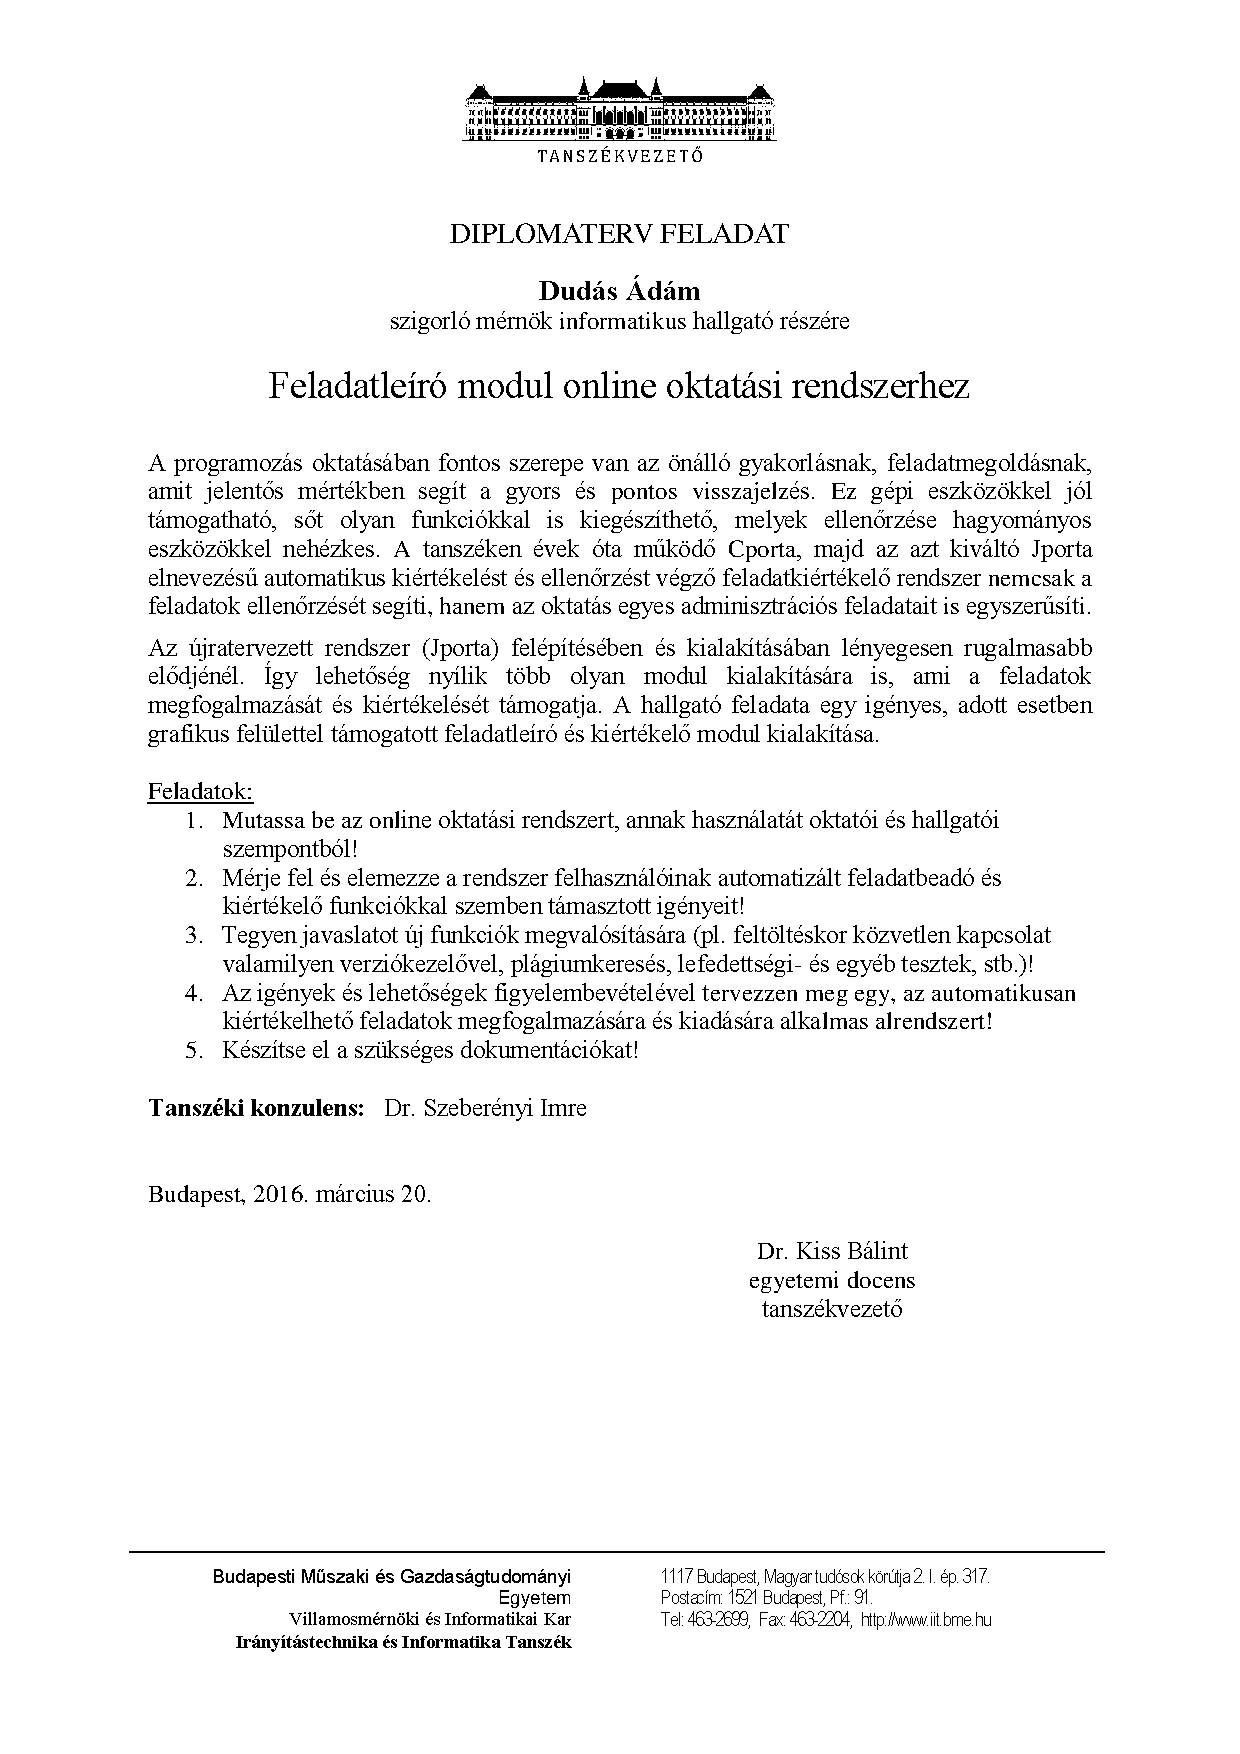
\includepdf[pages={1}]{feladatkiiras.pdf}
%--------------------------------------------------------------------------------------
%	The title page
%--------------------------------------------------------------------------------------
\begin{titlepage}
\begin{center}

\includegraphics[width=60mm,keepaspectratio]{figures/BMElogo.png}\\
\vspace{0.3cm}
\textbf{Budapesti M�szaki �s Gazdas�gtudom�nyi Egyetem}\\
\textmd{Villamosm�rn�ki �s Informatikai Kar}\\
\textmd{\viktanszek}\\[5cm]

\vspace{0.4cm}
{\huge \bfseries \vikcim}\\[0.8cm]
\vspace{0.5cm}
\textsc{\Large \vikdoktipus}\\[4cm]

\begin{tabular}{cc}
 \makebox[7cm]{\emph{K�sz�tette}} & \makebox[7cm]{\emph{Konzulens}} \\
 \makebox[7cm]{\vikszerzo} & \makebox[7cm]{\vikkonzulens}
\end{tabular}

\vfill
{\large \today}
\end{center}
\end{titlepage}



%--------------------------------------------------------------------------------------
% Nyilatkozat
%--------------------------------------------------------------------------------------
\begin{center}
\large
\textbf{HALLGAT�I NYILATKOZAT}\\
\end{center}

Alul�rott \emph{\vikszerzo}, szigorl� hallgat� kijelentem, hogy ezt a szakdolgozatot/ diplomatervet \textcolor{blue}{(nem k�v�nt t�rlend�)} meg nem engedett seg�ts�g n�lk�l, saj�t magam k�sz�tettem, csak a megadott forr�sokat (szakirodalom, eszk�z�k stb.) haszn�ltam fel. Minden olyan r�szt, melyet sz� szerint, vagy azonos �rtelemben, de �tfogalmazva m�s forr�sb�l �tvettem, egy�rtelm�en, a forr�s megad�s�val megjel�ltem.

Hozz�j�rulok, hogy a jelen munk�m alapadatait (szerz�(k), c�m, angol �s magyar nyelv� tartalmi kivonat, k�sz�t�s �ve, konzulens(ek) neve) a BME VIK nyilv�nosan hozz�f�rhet� elektronikus form�ban, a munka teljes sz�veg�t pedig az egyetem bels� h�l�zat�n kereszt�l (vagy autentik�lt felhaszn�l�k sz�m�ra) k�zz�tegye. Kijelentem, hogy a beny�jtott munka �s annak elektronikus verzi�ja megegyezik. D�k�ni enged�llyel titkos�tott diplomatervek eset�n a dolgozat sz�vege csak 3 �v eltelte ut�n v�lik hozz�f�rhet�v�.

\begin{flushleft}
\vspace*{1cm}
Budapest, \today
\end{flushleft}

\begin{flushright}
 \vspace*{1cm}
 \makebox[7cm]{\rule{6cm}{.4pt}}\\
 \makebox[7cm]{\emph{\vikszerzo}}\\
 \makebox[7cm]{hallgat�}
\end{flushright}
\thispagestyle{empty}

\vfill
\clearpage
\thispagestyle{empty} % an empty page


\tableofcontents\vfill
%----------------------------------------------------------------------------
% Abstract in hungarian
%----------------------------------------------------------------------------
\chapter*{Kivonat}\addcontentsline{toc}{chapter}{Kivonat}

A tanulási folyamatban jelentős szerep jut az önálló gyakorlásnak, feladatmegoldásnak, amelyhez fontos, hogy eredményességéről minél gyorsabb és megbízhatóbb visszajelzést kapjon a tanuló.
Ezt nagyban segítheti, ha a szükséges ellenőrzések minél nagyobb része automatizáltan történik, sok munkát levéve ezzel az oktatók válláról.
A programozás oktatása ebből a szempontból kitüntetett helyzetben van, hiszen a programok helyességének, elvárt működéstől való eltéréseinek vizsgálata már szinte a kezdetektől magas fokú automatizálással történik.

Az utóbbi időben, az online oktatás lehetőségeinek felismerésével, a szélessávú internethozzáférések mindenki számára elérhetővé válásával elterjedtté váltak az oktatást segítő platformok, melyek a hallgatók és az oktatók munkáját a tantermeken kívül is segítik.
Ilyen rendszer a BME Irányítástechnika és Informatika Tanszékén működő JPORTA is, amely a programozás oktatását automatikus feladatkiértékelést és ellenőrzést végző funkciója mellett egyéb adminisztrációs oktatói feladatok támogatásával igyekszik segíteni.

Diplomatervemben bemutatom a JPORTA rendszer működését, és a már említett feladatkiértékelő alrendszer tervezésének lépéseit.
Ez utóbbi részeként ismertetem a modullal szemben támasztott követelményeket, és ez alapján megtervezek egy, az automatizáltan kiértékelhető feladatok leírására alkalmas struktúrát, és az ezzel elkészített feladatokra érkező, hallgatók által készített megoldások kiértékelésére képes rendszert.
Végül javaslatot teszek két új funkció megvalósítására, melyeket röviden részletezek.
\vfill

%----------------------------------------------------------------------------
% Abstract in english
%----------------------------------------------------------------------------
\begin{otherlanguage}{english}
\chapter*{Abstract}\addcontentsline{toc}{chapter}{Abstract}

There is a considerable part in the process of learning that goes to individual practice and problem solving where getting fast and reliable feedback about their progress is essential for students.
This can benefit greatly from doing substancial parts of the necessary verification automatically, freeing educators from significant work.
From this perspective the education of programming is in a special position because validation and testing of programs was performed with high levels of automation from the beginning.

In recent times, with the recognition of potential in online education and the widespread availability of broadband internet connectivity we see the proliferation of platforms supporting education that aid the work of students and teachers outside of the classroom.
JPORTA found at the Department of Control Engineering and Information Technology at BUTE is such a system providing assistance for educators with administrative tasks beside its automatic submisson evaluation and testing facility.

In my master's thesis I'll introduce the operation of JPORTA and the design process of the aformetioned submission evaluation subsystem.
As part of this, I'll present the requirements for the module, than I'll design a structure suitable for the description of automatically evaluable assignments and a system capable of evaluating submissions made by students for assignments created via said structure.
Lastly, I'll suggest two new features which I'll detail briefly.
\end{otherlanguage}
\vfill


%----------------------------------------------------------------------------
\chapter{Bevezető}
%----------------------------------------------------------------------------

% Gyakorlás szerepe a tanulásban
A tanulás egy nehéz és időigényes folyamat, melynek megértésével és tökéletesítésével napjainkban is aktívan foglakozik a tudomány.
Ennek a folyamatnak elengedhetetlen része az önállóan végzett feladatmegoldás, a gyakorlás, mely során az elméleti tudás a gyakorlatban is hasznosítható tapasztalattá válik.
Gyakorlás közben fontos, hogy minél gyakrabban -- ha lehet, folyamatosan -- ellenőrizzük munkánk eredményét, ezzel biztosítva azt, hogy ne keletkezzenek rossz berögződések, melyek utólagos kijavítása további időt igényelne.

Az ellenőrzés módozatait többféle nézőpontból is értékelhetjük.
Az egyik ilyen nézőpont az ellenőrzési módszer flexibilitása, amely azt mutatja meg, mennyire változtatható meg a feladat úgy, hogy az ellenőrzési módszer továbbra is alkalmazható maradjon.
A spektrum egyik végén állnak az inflexibilis módszerek, amilyen például egy adott feladathoz mellékelt megoldókulcs.
A legegyszerűbb megoldókulcsok egyedül a feladat elvárt eredményét adják meg, ezért ezek flexibilitása igen csekély, hiszen a feladatban bármilyen érdemi változtatást elvégezve elvesztik érvényességüket. 
Ugyanakkor ezek a leggyorsabb és legolcsóbb módszerek, hiszen egyetlen összehasonlítás szükséges a saját és a megoldókulcs által megadott érték között, a megoldókulcsok pedig minimális költséggel sokszorosíthatóak és felhasználhatóak.
A spektrum másik végén találhatóak az oktatók -- általános esetben az adott terület szakértői --, akik a feladat témakörében való jártasságuk révén gyakorlatilag bármely megoldás ellenőrzésére képesek.
Az oktató azonban drága erőforrás, mind időben, mind pénzben, hiszen egy adott téma szakértőjeként a tanulók feladatainak ellenőrzése helyett az iparban is nagy szükség lenne rá.
Ebből fakadóan -- sok oktató alkalmazása költséges, ugyanakkor az iparnak nagyszámú szakértőre van szüksége -- az egy oktatóra eső hallgatók száma igen magas, amely körülmény nem kedvez az oktatás színvonalának, hiszen így minden hallgatóra kevesebb ideje jut az oktatónak.
Ha a spektrum két végének előnyeit -- könnyű sokszorosíthatóság, gyors működés, de magasabb szintű flexibilitás szakértelem hozzáadásával -- összehozzuk a számítástechnika által nyújtott automatizálási lehetőségekkel, eljuthatunk az \textit{automatizált feladatkiértékelő rendszerek} ötletéhez.


\section{Automatizált feladatkiértékelés}

\section{Online oktatást segítő rendszerek}
% TODO: Feladat indokoltsága: miért/mire jók az online oktatási rendszerek, a feladatbeadó rendszerek, automatikus kiértékelés
%       Eddigi megoldások (Coursera, Khan Academy, edX, Cporta)[http://www.lifehack.org/articles/money/25-killer-sites-for-free-online-education.html], hallgatói és oktatói szemszög


\section{A diplomaterv felépítése}
A dolgozatot az elvégzett munka és továbbfejlesztési lehetőségek összefoglalásával zárom.

%----------------------------------------------------------------------------
\chapter{Tervezés}
%----------------------------------------------------------------------------

% Jporta funkciói, felépítése, technológiák (Python 3, Django, Celery, RabbitMQ (AMQP, routing)), vizuális nyelvek (?), fejlesztési célok (igények)

% Javaslat új funkció(k)ra (?) (pl. csapatrendszer)

% Feladatkészítés menete
% Feladatkiadás
% Feladatbeadás
% Feladatkiértékelés
%----------------------------------------------------------------------------
\chapter{Megvalósítás}
%----------------------------------------------------------------------------

% Feljlesztés menete: git, Vim, CIRCLE devenv
% Megvalósítás: felhasznált technológiák beágyazása a leírásba, szemléltető ábrák
%----------------------------------------------------------------------------
\chapter*{Összefoglalás}\addcontentsline{toc}{chapter}{Összefoglalás}
%----------------------------------------------------------------------------

A megtervezett műszaki alkotás értékelése, kritikai elemzése, továbbfejlesztési lehetőségek

\section*{További fejlesztések}\addcontentsline{toc}{section}{További fejlesztések}
%----------------------------------------------------------------------------
\chapter*{Köszönetnyilvánítás}\addcontentsline{toc}{chapter}{Köszönetnyilvánítás}
%----------------------------------------------------------------------------

Szeretnék köszönetet mondani konzulensemnek, Dr.~Szeberényi Imrének, aki tanulmányaimban és munkám során is támogatott engem -- és rajtam kívül még egy másik tucat hallgatót -- áldozatos munkájával.  

Külön köszönet jár kollégámnak, Kálmán Viktornak, akivel vállvetve dolgoztunk a Jporta rendszer tervezésén és megvalósításán, és aki nélkül a Jporta kezelői felületének ergonómiája egy kaktuszéval vetekedne.

Köszönet illeti Őry Mátét és Guba Sándort, akiknek a Jporta alapjainak lerakásában volt fontos szerepe, valamint a BME IK többi munkatársát, akik kellemesebbé tették a munkával eltöltött időt.

Végül, de nem utolsó sorban, szeretném megköszönni édesapámnak, Dr.~Dudás Lászlónak és páromnak, Szabó Katalinnak, hogy a munka és jelen dolgozat megírása alatt végig segítettek és támogattak. 
\listoffigures\addcontentsline{toc}{chapter}{Ábrák jegyzéke}
\listoftables\addcontentsline{toc}{chapter}{Táblázatok jegyzéke}
%\printglossary[title=Rövidítések jegyzéke]

\bibliography{bibliography}\addcontentsline{toc}{chapter}{Irodalomjegyzék}
\bibliographystyle{huplain}

\label{page:last}
\end{document}
